\documentclass[
  article,
  12pt,
  oneside,
  a4paper,
  english,
  brazil,
  chapter=TITLE,
  section=TITLE,
  subsection=TITLE
]{abntex2}

\usepackage[T1]{fontenc}
\usepackage[utf8]{inputenc}
\usepackage{newtxtext,newtxmath}
\usepackage{indentfirst}
\usepackage{graphicx}
\usepackage{microtype}
\usepackage{placeins}
\usepackage{listingsutf8}

\lstset{
  inputencoding=utf8/latin1,
  language=Python,
  basicstyle=\ttfamily\footnotesize,
  breaklines=true,
  columns=fullflexible,
  keepspaces=true,
  showstringspaces=false,
  tabsize=2,
  frame=single,
  numbers=left,
  numberstyle=\tiny,
  numbersep=8pt,
  xleftmargin=2em,
  framexleftmargin=1.6em,
  aboveskip=8pt,
  belowskip=8pt
}

\makeatletter
\g@addto@macro{\UrlBreaks}{\do\_}
\makeatother

\titulo{Classificação do impacto das redes sociais com k-NN}
\autor{Ian de Araújo \and Jardson Alan}
\local{Rio Grande do Norte}
\data{2026}
\instituicao{%
  Instituto Federal de Educação, Ciência e Tecnologia\\
  do Rio Grande do Norte%
}
\preambulo{%
  Artigo apresentado à disciplina de Análise de Dados do Instituto Federal
  de Educação, Ciência e Tecnologia do Rio Grande do Norte, com o registro
  da etapa de classificação com k-vizinhos mais próximos.%
}

\hypersetup{
  hidelinks,
  pdftitle={Classificação do impacto das redes sociais com k-NN},
  pdfauthor={Ian de Araújo; Jardson Alan}
}

\renewcommand{\imprimircapa}{%
  \begin{capa}%
    \SingleSpacing
    \begin{center}
      \imprimirinstituicao\par
      \vspace*{\fill}
      \imprimirautor\par
      \vspace*{\fill}
      {\bfseries\imprimirtitulo\par}
      \vspace*{\fill}
      \imprimirlocal\par
      \imprimirdata\par
    \end{center}
    \vspace*{1cm}
  \end{capa}%
}

\renewcommand{\folhaderostocontent}{%
  \SingleSpacing
  \begin{center}
    \imprimirautor\par
  \end{center}
  \vspace{3.2cm}
  \begin{center}
    {\bfseries\imprimirtitulo\par}
  \end{center}
  \vspace{2.2cm}
  \hfill
  \begin{minipage}[t]{.46\textwidth}
    \imprimirpreambulo
  \end{minipage}
  \vspace{3.2cm}
  \begin{center}
    \imprimirlocal\par
    \imprimirdata\par
  \end{center}
}

\AtBeginDocument{%
  \setlength{\absleftindent}{0pt}%
  \setlength{\absrightindent}{0pt}%
  \setlength{\absparindent}{0pt}%
  \setlength{\emergencystretch}{2.5em}%
}

\graphicspath{{../figures/}}

\begin{document}

\pretextual
\imprimircapa
\imprimirfolhaderosto

\textual

\begin{center}
  \bfseries\imprimirtitulo
\end{center}

\vspace{0.75\baselineskip}
\noindent Ian de Araújo\footnotemark{} e Jardson Alan\footnotemark[\value{footnote}]
\footnotetext{Estudantes da disciplina de Análise de Dados do Instituto Federal de Educação, Ciência e Tecnologia do Rio Grande do Norte.}

\begin{resumo}
Esta etapa classifica o impacto das redes sociais em 4.500 estudantes com o algoritmo k-vizinhos mais próximos (k-NN). A classe é \texttt{Overall\_Impact}, com os rótulos \texttt{Beneficial}, \texttt{Neutral} e \texttt{Negative}. As entradas são as sete medidas numéricas padronizadas do agrupamento, e o índice de saúde mental fica de fora. O valor de k é escolhido por \texttt{GridSearchCV}, no recorte de treino, entre os ímpares de 1 a 31. O melhor valor foi k = 3. Com ele, a validação cruzada de cinco partes, feita por \texttt{cross\_val\_score}, dá acurácia média de 0,9444. O resultado fica acima do Naive Bayes (0,9238) e pouco abaixo da árvore de decisão (0,9480).

\vspace{\onelineskip}
\noindent
\textbf{Palavras-chave}: Classificação. k-NN. Validação cruzada. Redes sociais.
\end{resumo}

\section{Etapa de classificação com k-NN}

O objetivo é prever a classe já existente em \texttt{Overall\_Impact}, como nos outros classificadores. Há 3.681 registros \texttt{Beneficial}, 654 \texttt{Neutral} e 165 \texttt{Negative}. O arquivo é \texttt{data/raw/}\allowbreak\texttt{dataset.csv}, com 4.500 estudantes (YADAV, 2026).

O k-NN classifica um registro pela votação dos k exemplos de treino mais próximos, com distância euclidiana. Por usar distância, ele é sensível à escala dos atributos. Por isso as entradas vêm de \texttt{prepare\_data}, em \texttt{src/clustering/}\allowbreak\texttt{grouping.py}, que já preenche os vazios de estresse e de GPA com a média truncada por idade e padroniza as sete colunas numéricas. \texttt{Student\_ID} e \texttt{Mental\_Health\_Index} não entram, e a classe também não.

O recorte é o mesmo dos outros classificadores, com 33\% dos registros para teste e semente 125. A comparação feita pela etapa é a validação cruzada de cinco partes, com acurácia, aplicada por \texttt{cross\_val\_score}.

\section{Escolha de k com GridSearchCV}

O \texttt{GridSearchCV} testa k = 1, 3, 5, \ldots, 31 só no recorte de treino, com cinco partes internas e acurácia como critério. Os valores são ímpares para evitar empates na votação. O melhor foi k = 3, com acurácia média de 0,9516 na busca. A Figura~\ref{fig:k} mostra a curva. Com k = 1 a acurácia cai para cerca de 0,935. De k = 3 em diante ela fica entre 0,947 e 0,952, e as diferenças entre esses valores são menores que o desvio-padrão entre as partes.

\begin{figure}[htb]
  \centering
  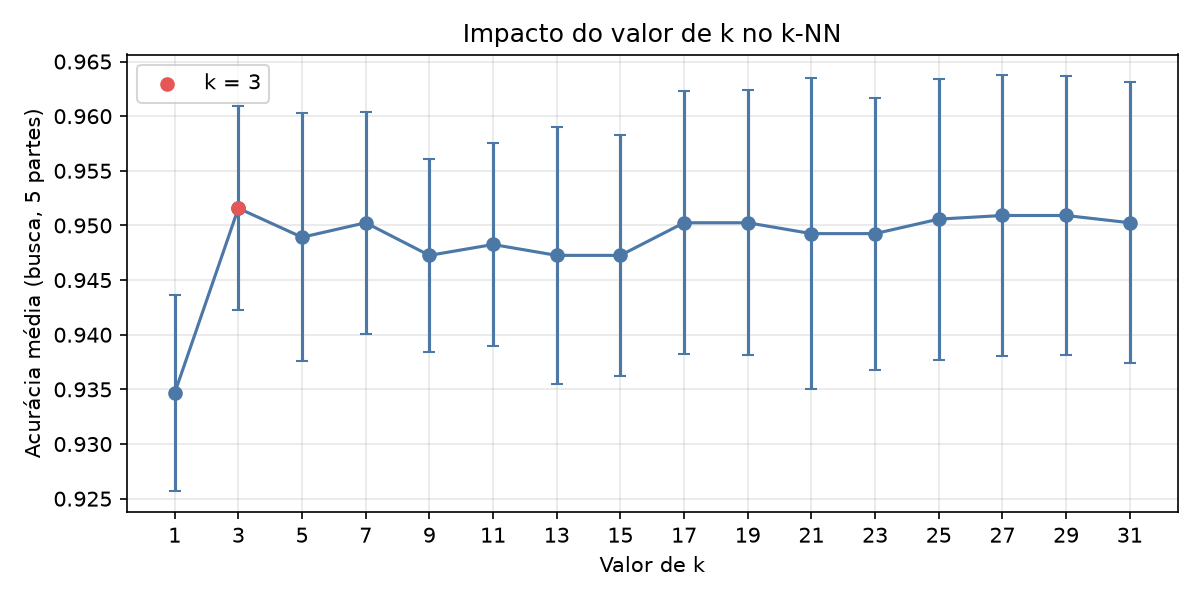
\includegraphics[width=0.9\textwidth]{knn_k_selection.png}
  \caption{Acurácia média da busca para cada valor de k}
  \label{fig:k}
  \fonte{Elaborado pelos autores (2026), pela execução do classificador.}
\end{figure}

\section{Desempenho}

Um k-NN novo, com k = 3, foi avaliado por \texttt{cross\_val\_score} no conjunto inteiro. A média foi 0,9444, com desvio-padrão de 0,0065. A Tabela~\ref{tab:cv} compara as cinco partes com os outros dois classificadores e a Figura~\ref{fig:cv} mostra os mesmos valores.

\begin{table}[htb]
  \centering
  \caption{Acurácia na validação cruzada de cinco partes}
  \label{tab:cv}
  \small
  \begin{tabular}{lrrrrrr}
    \toprule
    Modelo & Parte 1 & Parte 2 & Parte 3 & Parte 4 & Parte 5 & Média \\
    \midrule
    Naive Bayes & 0,9278 & 0,9289 & 0,9233 & 0,9067 & 0,9322 & 0,9238 \\
    Árvore de decisão & 0,9544 & 0,9444 & 0,9556 & 0,9356 & 0,9500 & 0,9480 \\
    k-NN (k = 3) & 0,9522 & 0,9378 & 0,9511 & 0,9444 & 0,9367 & 0,9444 \\
    \bottomrule
  \end{tabular}
  \fonte{Elaborado pelos autores (2026), pela execução dos classificadores.}
\end{table}

\begin{figure}[htb]
  \centering
  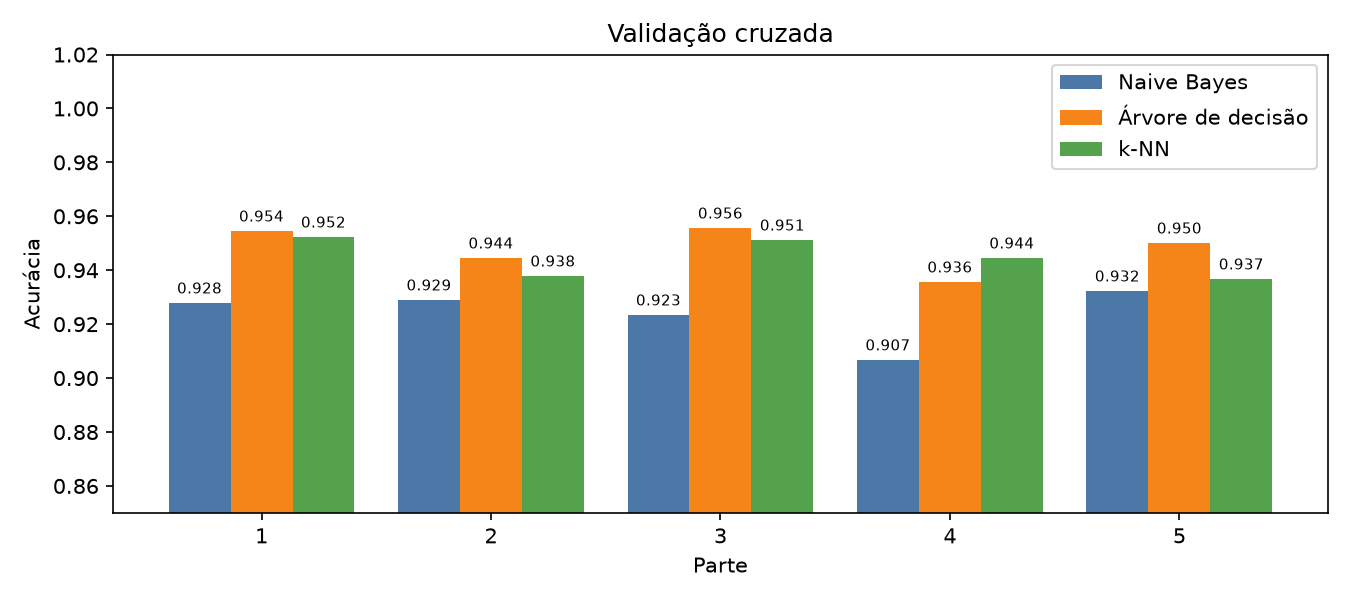
\includegraphics[width=\textwidth]{knn_cross_validation.png}
  \caption{Acurácia nas cinco partes da validação cruzada}
  \label{fig:cv}
  \fonte{Elaborado pelos autores (2026), pela execução dos classificadores.}
\end{figure}

No recorte de teste, a acurácia foi 0,9401 e a área sob a curva ROC, em média macro um contra os demais, foi 0,9422. A Tabela~\ref{tab:knn} é a matriz do teste. O k-NN acerta 1.181 dos 1.204 \texttt{Beneficial}, 38 dos 52 \texttt{Negative} e 177 dos 229 \texttt{Neutral}. O recall de \texttt{Negative} (0,73) é o mais baixo dos três classificadores: 14 desses registros foram previstos como \texttt{Neutral}.

\begin{table}[htb]
  \centering
  \caption{Matriz do k-NN no recorte de teste}
  \label{tab:knn}
  \begin{tabular}{lrrr}
    \toprule
    Real & Beneficial & Negative & Neutral \\
    \midrule
    Beneficial & 1181 & 0 & 23 \\
    Negative & 0 & 38 & 14 \\
    Neutral & 42 & 10 & 177 \\
    \bottomrule
  \end{tabular}
  \fonte{Elaborado pelos autores (2026), pela execução do classificador.}
\end{table}

\begin{figure}[htb]
  \centering
  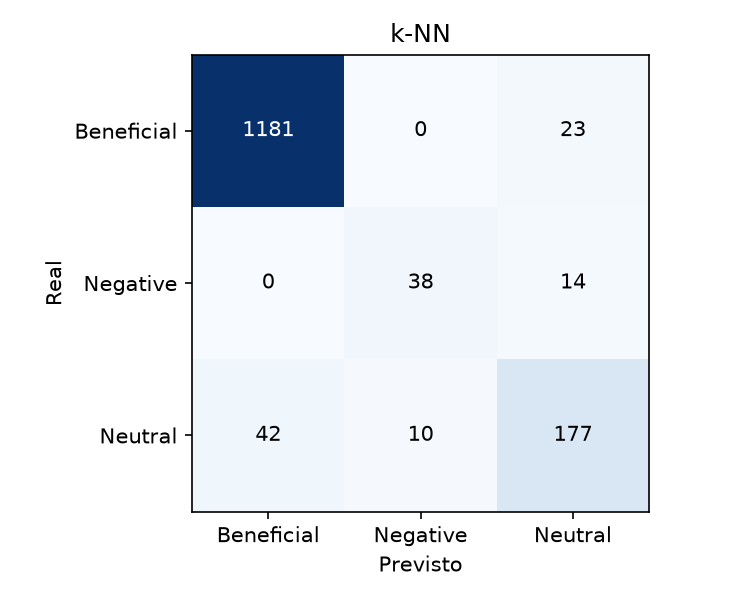
\includegraphics[width=0.6\textwidth]{knn_confusion_matrix.png}
  \caption{Matriz de confusão do k-NN no recorte de teste}
  \label{fig:matriz}
  \fonte{Elaborado pelos autores (2026), pela execução do classificador.}
\end{figure}

\section{Comparativo}

Pela média da validação cruzada, a árvore de decisão (0,9480) fica pouco acima do k-NN (0,9444), e os dois ficam bem acima do Naive Bayes (0,9238). A diferença entre árvore e k-NN, de 0,0036, é menor que o desvio-padrão das partes, e o k-NN supera a árvore na parte 4. Os três ficam acima da proporção da classe majoritária (81,8\%), mas a acurácia sozinha esconde as classes pequenas: o k-NN recupera menos \texttt{Negative} que o Naive Bayes (38 contra 49 acertos) e que a árvore (44). O k-NN tem o menor desvio-padrão entre os três, 0,0065.

\FloatBarrier

\section{Código utilizado}

As listagens são os arquivos desta etapa, como estão no repositório. \texttt{main.py} chama o classificador e a função que grava as figuras. \texttt{knn.py} escolhe o k com \texttt{GridSearchCV} e avalia o modelo escolhido com \texttt{cross\_val\_score}. \texttt{charts.py} grava os gráficos em \texttt{reports/figures/}.

\subsection{Chamada no fluxo}

Arquivo \texttt{main.py}.

\lstinputlisting{../../../main.py}

\subsection{k-NN}

Arquivo \texttt{src/classifiers/}\allowbreak\texttt{knn.py}.

\lstinputlisting{../../../src/classifiers/knn.py}

\subsection{Gráficos}

Arquivo \texttt{src/visualization/}\allowbreak\texttt{charts.py}.

\lstinputlisting{../../../src/visualization/charts.py}

\postextual

\begin{thebibliography}{9}
\bibitem{yadav2026}
YADAV, Harish. \textbf{Impact of Social Media on Life}. 2026. Conjunto de dados. Disponível em: \url{https://www.kaggle.com/datasets/harishyadav0506/impact-of-social-media-on-life}. Acesso em: 9 nov. 2026.
\end{thebibliography}

\end{document}
